\section{Specifiying LED behavior in Resolve}
\label{sec:specifiying}

In this section, we provide mathematical and programmatic elements of an LED strip component to give readers both a concrete look at the language, and introduce some new features aimed at making it more amenable to the development of embedded applications. Note that while we provide the level of detail necessary to understand the current example, readers interested in gaining a more complete, in depth knowledge of the language are encouraged to refer to \cite{sitaraman:2011, kulczycki:2008}.

\subsection{Concepts}
\label{ssec:concepts}
In RESOLVE, programs are composed of several different modules that range from interfaces and realizations, to client (facility) modules. The first we  discuss here, termed a \textit{concept}, defines a specification for a mathematical, abstract type. Similar to an interface in Java, a concept provides a number of operation signatures that implementors are expected to realize. Shown below is an \texttt{LED\_Template} concept that provides an LED light strip abstraction.

\begin{verbatim}
Concept LED_Template(eval Strip_Length: Integer);
    uses Boolean_Theory, String_Theory;
    requires 0 < Strip_Length 
	
    Type Family LED is modeled by Str(B);
        exemplar L;
        constraint |L| = Strip_Length;
        initialization ensures 
            ...
    
    Oper Set(updates L : LED; eval b : Boolean; 
                             eval i : Integer);
        requires 0 <= i < |L|;
        ensures L = (Prt_Btwn(0, i, #L) o <#b>) o
            Prt_Btwn(i, |#L|, #L) and |L| = |#L|;
    
    Oper Status(preserves L : LED; 
                        updates b : Boolean;
            eval i : Integer);
        requires 0 <= i < |L|;
        ensures Status = Element_At(i, #L);
        
end LED_Template;
\end{verbatim}

We model our conceptual LED strip using a mathematical string (finite sequence) of booleans, denoted \texttt{Str(B)}, where each boolean within the string indicates the status of that particular LED: On (true) or off (false). The \texttt{exemplar} clause located immediately below provides a handle to this abstract model, and is used throughout the remainder of the specification.

It's worth noting that unlike the \texttt{LED\_Template} presented in \cite{regula:2010} which models an LED as the \textit{cartesian product} of booleans $b_0$, $b_1$, \ldots , $b_4$, the strip model we present here instead uses strings for the following reasons:
\begin{itemize}
\item Strings are indexible, and thus do not require separate \texttt{Set} and \texttt{Status} operations for each individual LED.
\item This approach demonstrates the benefits of reusable mathematical theories. Indeed, the specifications listed here are based (almost) entirely in \texttt{String\_Theory} and are therefore able to make use of RESOLVE's pre-existing math libraries.
\end{itemize}

The concept provides two operations. The first, \texttt{Set}, takes as a parameter an instance of an LED strip \texttt{L}, a boolean \texttt{b}, and an integer \texttt{i}. The operation \texttt{requires} that \texttt{i} falls within the length of the strip, and \texttt{ensures} two things upon completion: The length of the outgoing strip \texttt{L} is the same as the incoming strip, \texttt{\#L}, and that the LED in position \texttt{i} of \texttt{L} is set to boolean \texttt{b}\footnote{Note that the \texttt{ensures} clause in this case is strong enough to assert that \textit{only} the boolean at location \texttt{i} has changed}. The \texttt{Status} operation is specified similarly. 

\subsection{Enhancements}

RESOLVE also allows users to extend the functionality provided by the base concept through \textit{enhancements} -- a form of specification inheritance. The enhancement we provide here, \texttt{Toggling\_Capability}, allows users to flip a specific LED to its complement.

Shown below is a specification for \texttt{Toggling\_Capability} and one particular realization of it.

\begin{verbatim}
Enhancement Toggling_Capability for LED_Template;

    Oper Toggle(upd L : LED; eval i : Integer);
        requires i >= 0 and i < |L|
        ensures L = (Prt_Btwn(0, i, #L) o  
                  <not(Element_At(i, #L))>) o
                  Prt_Btwn(i, |#L|, #L);
end Toggling_Capability;

Realization Toggling_Realiz for
            Toggling_Capability of LED_Template;

    Proc Toggle(upd L : LED; eval i : Integer);
        Var Flipped_Contents : Boolean;
        Status(L, Flipped_Contents, Replica(i));
        Set(L, Not(Flipped_Contents), Replica(i));
    end Toggle;
    
end Toggling_Realiz;
\end{verbatim}

The enhancement specifies a single operation, \texttt{Toggle}, which states that upon termination, the LED located at position \texttt{i} in \texttt{L} is the complement of that same location in the incoming LED, \texttt{\#L}.

Note that the enhancement specifications themselves look and function largely the same as a normal concept: Each specifies a purely conceptual module, and hence is implementation neutral. 

Enhancement realizations are similar in the sense that any operation called within the context of an enhancement realization refers to the operation specified in the concept -- meaning no knowledge of its implementation details are required.

\subsection{Verification}

We now turn to the task of verifying our small toggling enhancement. The first step in doing so is to generate Verification Conditions (VCs) for \texttt{Toggle\_Realiz}, which, if proven, will establish the correctness of this particular implementation. One thing to note about the VCs themselves is that they are generated from specific lines of a realization, and exist to ensure that the content of the realization is consistent with its specification: This entails checking for array access violations, parameters not meeting preconditions, etc.  

\begin{figure}[!htb]
\centering
\begin{tabular}{lccc}
	\toprule
	Condition \# & Time (ms)	& Steps	& Search \\
	\midrule
	VC 0\_1	& 7009	& 6	& 0	\\
	VC 0\_2	& 5185	& 5	& 0	\\
	VC 0\_3	& 3354	& 6	& 0	\\
	VC 0\_4	& 4810	& 5	& 0	\\
	VC 0\_5	& 7133	& 5	& 0	\\
	\bottomrule
\end{tabular}
\caption{Verification results for operation \texttt{Toggle}}
\label{fig:results}
\end{figure}

As the results summarized in Figure \ref{fig:results} indicate, using RESOLVE's integrated prover, we are able to mechanically and automatically dispatch all VCs for \texttt{Toggling\_Realiz}, thus verifying its correctness. In terms of proof difficulty, given the number of steps and time taken to establish each goal, we conclude that the VCs generated are of a straightforward variety. Readers interested however in learning more about the steps and specific actions the prover takes in transforming givens and dispatching similar (and more complex) VCs should refer to \cite{smith:2013}.

\subsection{Facilities}
\label{sec:facilities}

With our formally specified LED strip component in place -- and a verified enhancement on this component -- we now turn to a small embedded application that combines these elements to iteratively toggle the lights within an LED strip.

Shown below is a RESOLVE facility module that implements the client logic of this embedded application.
\begin{verbatim}
Facility LED_Telos_Demo;
    uses Std_Clock_Fac, Std_Boolean_Fac, 
            Std_Integer_Fac;
    
    Facility LED_Fac is LED_Template(3)
        externally realized by Std_LED_Realiz
     enhanced by Toggling_Capability
        realized by Toggling_Realiz;
        
    Operation Main(); Procedure
    
        (* Declare LED strip indices *)
        Var I0, I1, I2 : Integer;
        Var Loop : Boolean;
        
        (* Declare an LED strip *)
        Var L : LED;
        
        I0 := 0; I1 := 1; I2 := 2;
        
        Loop := True();
        While(Loop)
            changing Loop;
            maintaining ...
        do
            LED_Fac.Toggle(L, I0);
            Std_Clock_Fac.Wait_500_Milli_Seconds();
            
            LED_Fac.Toggle(L, I1);
            Std_Clock_Fac.Wait_500_Milli_Seconds();
            
            LED_Fac.Toggle(L, I2);
            Std_Clock_Fac.Wait_500_Milli_Seconds();
        end;
    end Main;
    
end LED_Telos_Demo;
\end{verbatim}

Prior to using the LED component developed in the previous sections, we first must bind our \texttt{LED\_Template} specification with an appropriate realization. This is accomplished via the facility declaration located directly beneath the \texttt{uses} clause, which pairs the specification (\texttt{LED\_Template}) with a realization (\texttt{Std\_Led\_Realiz}). Note that the ability to toggle is added \textit{on top} of this facility declaration in a similar fashion. The remaining bulk of logic driving the application rests in the non terminating busy loop inside operation \texttt{Main}, where we use our enhancement-provided \texttt{Toggle} operation to successively turn each LED within the strip on, then off.

\subsection{``External'' Realization Support}
\label{ssec:external}

\begin{figure*}[!htb]
\centering
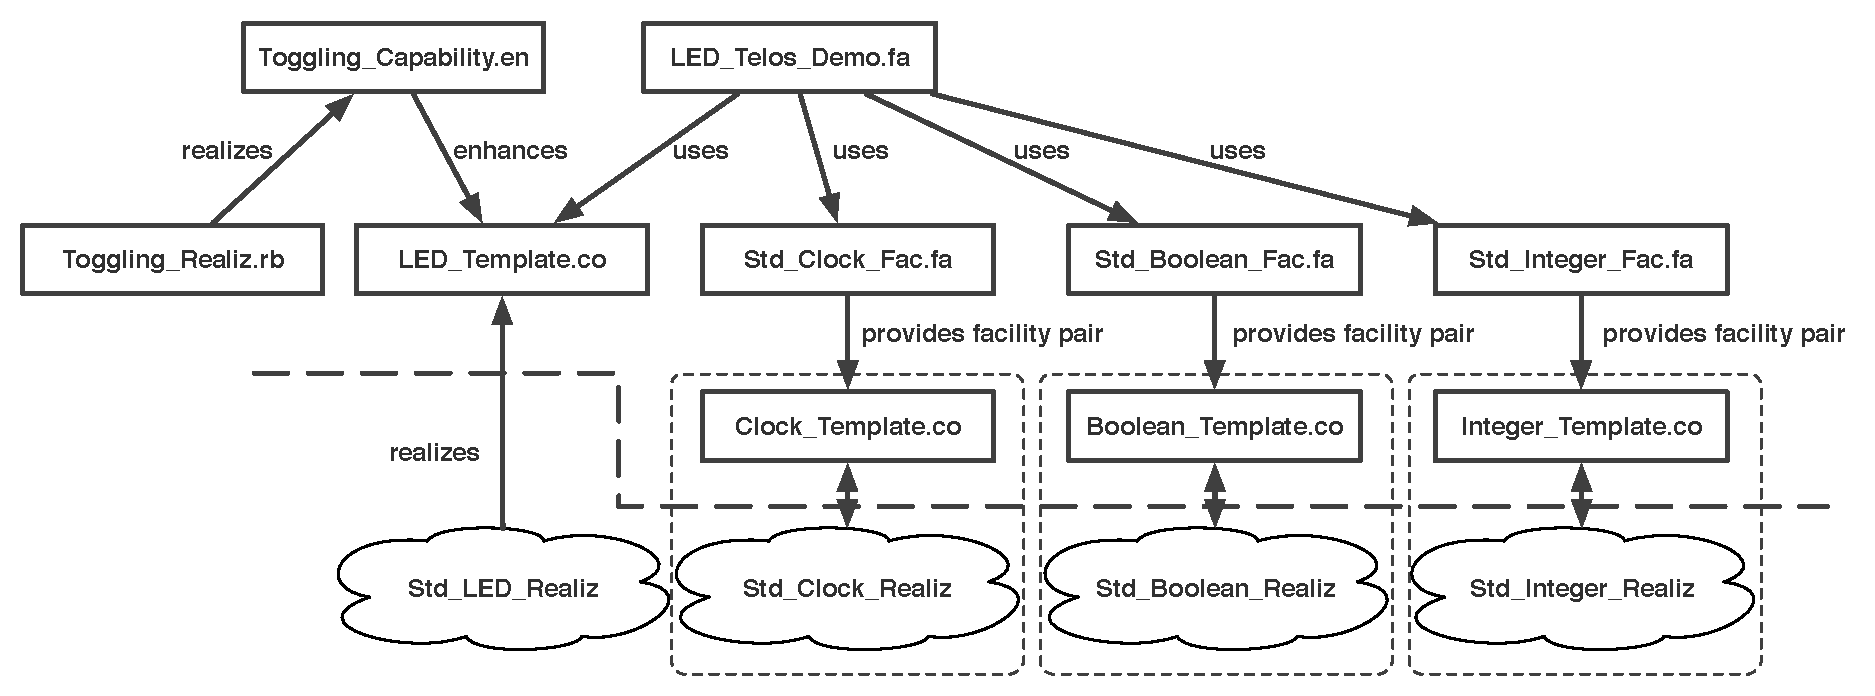
\includegraphics[scale=.55]{figs/component_graph.pdf}
\caption{A diagram illustrating inter-component relationships for the example detailed in Section 3. Files displayed in clouds indicate externally realized components, while dotted line separating these from others indicates the current boundary between low-level, hardcoded components, and native RESOLVE abstractions.}
\end{figure*}
\label{fig:imp}


Readers might note that we never presented a realization of \texttt{LED\_Template}. Indeed, after having written the concept, the RESOLVE programmer would ideally provide a verifiable, native RESOLVE implementation. However, as our target platform is embedded, and our concept aims to provide control for LEDs -- a decidedly low level feature on embedded hardware -- our realization is forced to operate at similarly low levels by directly manipulating hardware pins provided by the msp430's chipset. 

RESOLVE, however, in its current state is too high level of a language to perform these tasks directly -- meaning it lacks the appropriate driver and language support to do so. In an effort to address this, we introduce the notion of \textit{external realizations}, which allow users to write their own realization of a concept in a language of their choosing.

The \texttt{LED\_Telos\_Demo} facility above demonstrates these developments through its use of the ``\texttt{externally realized}" phrase. This signals to the RESOLVE compiler that the user is providing a non-native realization of \texttt{LED\_Template}, with the expectation that it conforms to the specifications dictated in the concept. 

% Applies to base types in resolve as well

% Similar to NesC, the towers of abstraction idea... eventually, similar to nesc, we get enough abstraction  through machinery such as enhancements, etc to with pieces built on top of these externally realized components.

% gives flexibility to those wishing to write other drivers and new 

We feel this new keyword is beneficial for the following reasons:
\begin{itemize}
\item The language no longer must ``hide" the fact that some of the lower level components relied upon are not written in straight-line, native RESOLVE. The ``externally" keyword now transparently indicates this.
\item Provides flexibility for those users looking to wrap their low-level programs/drivers with formal RESOLVE interface specifications.
\end{itemize}

In the context of embedded systems, these developments are especially useful as we can now write custom, low level  drivers of the sort required for most embedded applications (e.g. LED strip drivers) while still providing extensible, formally specified interfaces. It is our hope and intention that new (native) RESOLVE components will be layered on top of these low level, externally realized (yet specified) drivers -- eventually reaching a level of abstraction where we can concern ourselves exclusively with verified, native RESOLVE components.

%In a very real sense, gives the language the capability of specifying its foundational components flexibly, and transparently which can later have all native RESOLVE components added on top. 

%More than givingHaving the freedom to use RESOLVE's specificational capabilities 

%mention performance stuff in future work section.